\documentclass[10pt]{beamer}

\usetheme[progressbar=frametitle,sectionpage=none]{metropolis}
\usepackage{appendixnumberbeamer}

\usepackage{booktabs}
\usepackage[scale=2]{ccicons}

\usepackage{pgfplots}
\usepgfplotslibrary{dateplot}

\usepackage{pgfgantt}
\usepackage{hyperref}

\usepackage[normalem]{ulem}

\usepackage{subcaption}

\usepackage{xspace}
\newcommand{\themename}{\textbf{\textsc{metropolis}}\xspace}

% \usepackage[romanian]{babel}
% \usepackage{fontspec}

\usepackage[backend=biber]{biblatex}
% \usepackage[numbers]{natbib}
\bibliography{../Final report/II2202-report.bib}

% \definecolor{white}{RGB}{255, 255, 255}
% \definecolor{black}{RGB}{0, 0, 0}
% \definecolor{softgray}{RGB}{240,240,240}
% \definecolor{gray}{RGB}{128,128,128}
\definecolor{oceanblue}{RGB}{0, 119, 190}

% \setbeamercolor{background canvas}{bg=white,fg=black}
% \setbeamercolor{normal text}{fg=black}
% \setbeamercolor{frametitle}{bg=white, fg=black}
\setbeamercolor{progress bar}{fg=oceanblue,bg=oceanblue}

% %For example blocks
% \setbeamercolor{block title example}{fg=red,bg=orange}
% \setbeamercolor{block body example}{fg=cyan,bg=yellow}

% %For alert blocks
\setbeamercolor{block title alerted}{fg=oceanblue}
% \setbeamercolor{block body alerted}{fg=black,bg=softgray}
\setbeamercolor{alerted text}{fg=oceanblue}

% %For blocks
% \setbeamercolor{block title}{fg=white,bg=blue}
% \setbeamercolor{block body}{fg=white,bg=green!40!black}


%\usepackage{grffile} % To remove filename from pdf figure

\newcommand{\resnettimebfc}{$5.79\pm0.022\%$}     % ( 5.82 +  5.82 +  5.66 +  5.82 +  5.81)/5
\newcommand{\resnettimecuda}{$5.29\pm0.006\%$}    % ( 5.26 +  5.29 +  5.27 +  5.31 +  5.32)/5     9.5% slower
\newcommand{\resnettimehalloc}{$not~working$}     %
\newcommand{\alexnettimebfc}{$41.62\pm0.001\%$}   % (41.61 + 41.66 + 41.60 + 41.61 + 41.61)/5
\newcommand{\alexnettimecuda}{$40.19\pm0.002\%$}  % (40.17 + 40.26 + 40.26 + 40.06 + 40.20)/5     3.6% slower
\newcommand{\alexnettimehalloc}{$36.31\pm0.011\%$}% 

% Pages
    \setbeamertemplate{footline}{%
       \raisebox{10pt}{\makebox[\paperwidth]{\hfill\makebox[30pt]{\scriptsize\insertframenumber\ / \inserttotalframenumber}}}}

\title{GPU Dynamic memory allocation algorithms for Machine Learning: A survey}
\author{Erik H. Wouters, Dragoş Ş. Perju \{\texttt{ehwo}$\mid$\texttt{dsperju}\}\texttt{@kth.se}}
\date{January 11, 2019}

\institute{KTH Royal University of Technology \quad Stockholm, Sweden}
% \titlegraphic{\hfill\includegraphics[height=1.5cm]{logo.pdf}}

\begin{document}

\maketitle

% Suggested slides (do not forget to number your slides):

%     Title slide: Project title[:subtitle], Name of student(s) who conducted the project, Date of the oral presentation (1 slide)
%     Problem statement, Why the problem is important to solve, and your Goals, problem context, [hypothesis], delimitations, ... (1 slide)
%     Background and Related work (b slides)
%     Method used to solve the problem (m slides)
%     Results and Analysis (r slides)
%     Conclusion (1 slide)
%     Future work (1 slide)
%     [Final slide - to solicit questions (1 slide)]

% I would suggest b ≤ 2, m ≤ 2, r ≤ 2, in any case b+m+r ≤ 6.

% \begin{frame}{Table of contents}
%   \setbeamertemplate{section in toc}[sections numbered]
%   \tableofcontents[hideallsubsections]
% \end{frame}

%\section{Introduction}

\begin{frame}[fragile]{Problem}

\metroset{block=fill}

\begin{exampleblock}{Problem context}
 \begin{itemize}
 \item Interest in dynamic memory allocation;
 \item Different applications use different allocators on the CPU only
     \begin{itemize}
         \item e.g.: \texttt{malloc}, \texttt{jemalloc}, etc.;
     \end{itemize}
 \item Different architectures (such as GPU) have different issues with allocating dynamically
     \begin{itemize}
         \item e.g.: \texttt{malloc} vs. \texttt{CudaMalloc}.
     \end{itemize}
 \end{itemize}
\end{exampleblock}
\end{frame}

% \begin{frame}[fragile]{The problem}

% \metroset{block=fill}

% \begin{alertblock}{Problem statement}
% % We believe that \textbf{machine learning} applications can benefit from using a scientifically chosen dynamic memory allocator, in order to have an improved performance.
%  We want to choose the best dynamic memory allocator when used with \textbf{TensorFlow}'s benchmark implementation of \textbf{ResNet-50}, in terms of overall speed, fragmentation and other metrics.
% \end{alertblock}
% \end{frame}

\begin{frame}[fragile]{Problem}

\metroset{block=fill}

\begin{alertblock}{Problem statement}
% We believe that \textbf{machine learning} applications can benefit from using a scientifically chosen dynamic memory allocator, in order to have an improved performance.
 We want to choose the best dynamic memory allocator when used with \textbf{TensorFlow}'s benchmark implementation of \textbf{ResNet-50} and \textbf{AlexNet}, in terms of overall speed (images per second).
\end{alertblock}

\begin{exampleblock}{Hypotheses}
\begin{enumerate}
\item TensorFlow allocates many smaller-sized objects, which \texttt{Halloc} favours in speed though its design.
\item Using \texttt{Halloc} with TensorFlow, which is described to be much faster than \texttt{CUDAMalloc} (3 to 3000 times) [2], will bring a performance improvement to the speed of TensorFlow's benchmark (images per second).
\item The configurable parameters of \texttt{Halloc} do not influence the speed of the benchmark.
\end{enumerate}

\end{exampleblock}

% \begin{exampleblock}{More specifically}
%  The memory allocation pattern of \textbf{TensorFlow}'s implementation of \textbf{ResNet-50} is not a great match for the memory allocator TensorFlow uses, we will investigate which previously published dynamic memory allocation algorithms perform better.
% \end{exampleblock}

\end{frame}

%     Background and Related work (b slides)
\begin{frame}[fragile]{Background}

\metroset{block=fill}

\begin{exampleblock}{Related work}
We extracted GPU memory allocator implementations from the source code of:

[1] \textit{M. Vinkler and V. Havran, “Register efficient dynamic memory allocator for GPUs” , Computer Graphics Forum, vol. 34, no. 8, pp. 143–154, 2015. [Online].} Available: \url{https://onlinelibrary.wiley.com/doi/abs/10.1111/cgf.12666}

TensorFlow uses NVIDIA CUDA as a GPU library, and \texttt{BFCAllocator} or \texttt{CUDAMalloc} as the primary dynamic GPU memory allocator.
\end{exampleblock}
\end{frame}

%     Method used to solve the problem (m slides)
\begin{frame}[fragile]{Background}

\metroset{block=fill}

\begin{alertblock}{GPU Dynamic memory allocation algorithms}
 \begin{itemize}
     \item \textbf{BFCMalloc} - Best-fit with coalescing;
     \item \textbf{CudaMalloc} - Proprietary algorithm of NVIDIA;
     \item \textbf{Halloc} - Hashing function used to reduce collision when many threads allocate. Favours small memory allocations.
 \end{itemize}
 Other allocators studied: \textbf{XMalloc}, \textbf{ScatterAlloc}, \textbf{FDGMalloc} -- all slower than \textbf{Halloc}. \textbf{CMalloc} has a design that does not favour small memory allocations.
\end{alertblock}

\begin{exampleblock}{TensorFlow CNN benchmark}
    \textbf{ResNet-50}, \textbf{AlexNet} - deep learning convolutional neural networks
\end{exampleblock}

\end{frame}

% \begin{frame}[fragile]{Background}
%  \begin{figure}
%  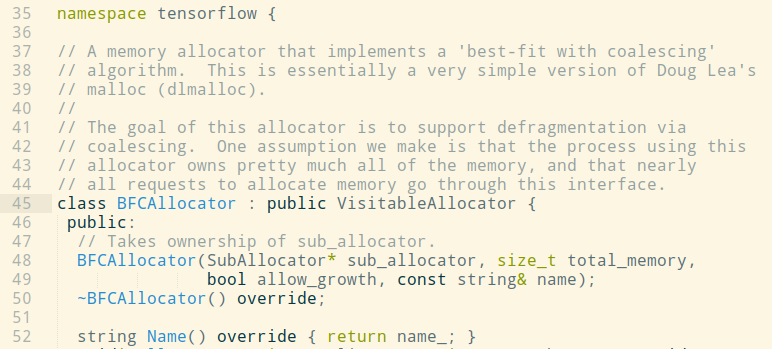
\includegraphics[scale=0.4]{images/BFCAllocator.png}
%  \caption{Exerpt from TensorFlow's source code, showing \texttt{BFCAllocator}}
%  \end{figure}
% \end{frame}

%\begin{frame}[fragile]{The problem}
%
%\metroset{block=fill}
%
%\begin{alertblock}{Problem statement}
% We believe that \texttt{BFCAllocator} is still unsuitable for TensorFlow and Convolutional %Neural Networks. We do not have a \textbf{hypothesis} yet, but we believe another allocation %algorithm can be mainly faster than \texttt{BFCAllocator}.
%\end{alertblock}
%
%\end{frame}

\begin{frame}[fragile]{Methodology}

\metroset{block=fill}

\begin{alertblock}{Methodology}
%Test different GPU dynamic memory allocation algorithms                           (such as: CudaMalloc and others);
% Benchmark such algorithms using a Machine Learning workload (TensorFlow CNN benchmarks).
\begin{enumerate}
    \item Analyze memory allocation pattern of \texttt{ResNet-50}, \texttt{AlexNet};
    \item Match pattern to memory allocator suggested by literature (\texttt{Halloc});
    \item Add \texttt{Halloc} allocator to TensorFlow source code;
    \item Use standard benchmarks on modified TensorFlow, to evaluate the performance compared to the built-in memory allocators;
    \item \texttt{Halloc} is configurable through different parameters -- evaluate performance by changing them systematically.
    
\end{enumerate}

\end{alertblock}
\end{frame}

% \begin{frame}[fragile]{Problem importance}

% \metroset{block=fill}

% \begin{exampleblock}{Why is the problem is important to solve}
% Improving allocation for \textbf{machine learning} means better performance for the same amount of time and the same amount of energy. 
% \end{exampleblock}

% \end{frame}

\begin{frame}[fragile]{Results and Analysis}

\metroset{block=fill}

\begin{figure}[!ht]
  \centering
  \begin{subfigure}[b]{0.49\textwidth}
    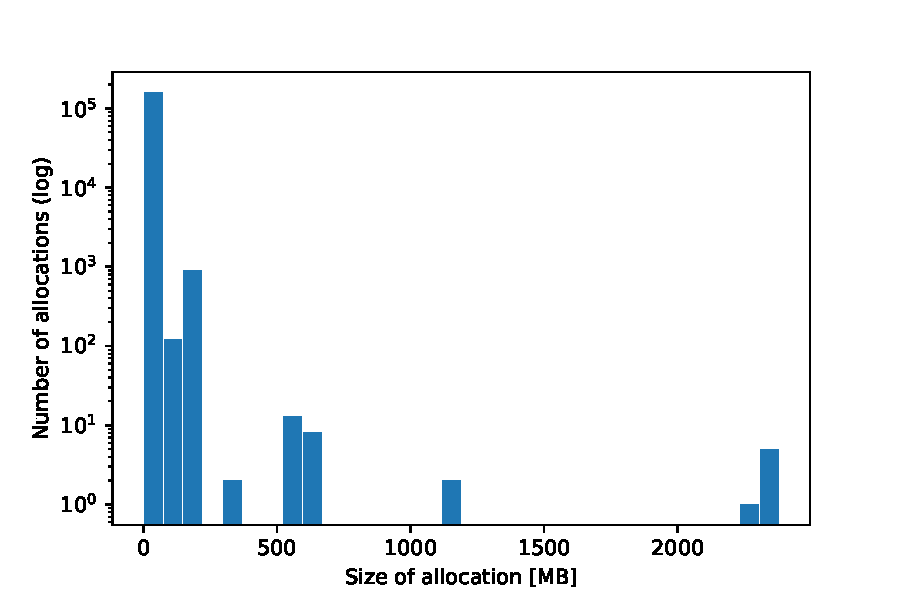
\includegraphics[width=\textwidth]{../Quantitative_Python/ResNet-50_hist_MB_ylog.pdf}
    \caption{ResNet-50}
  \end{subfigure}
  \begin{subfigure}[b]{0.49\textwidth}
    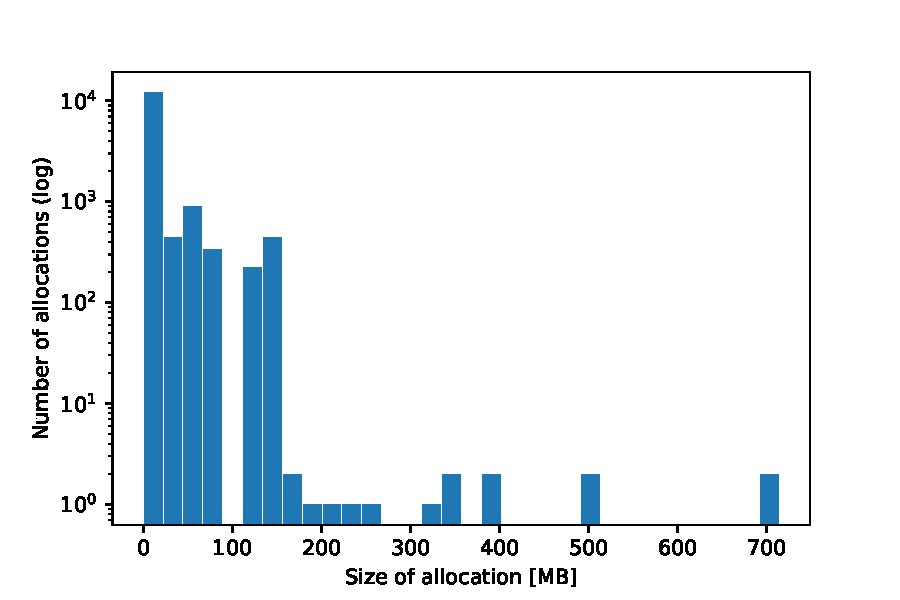
\includegraphics[width=\textwidth]{../Quantitative_Python/AlexNet_hist_MB_ylog.pdf}
    \caption{AlexNet}
  \end{subfigure}
  \caption{Histogram of object sizes requested for allocation for the two models ($32$ bins). Note that the number of allocations is depicted on a logarithmic scale, so each division is an order of magnitude.}
  \label{fig:hist}
\end{figure}

\end{frame}

%     Results and Analysis (r slides)
\begin{frame}[fragile]{Results and Analysis}

\metroset{block=fill}

\begin{exampleblock}{Benchmark Results}

    \begin{table}[!ht]
    \centering
    \caption{Benchmark Results}
    \label{tab:results}
    \begin{tabular}{|l|l|l|l|}
    \hline
    \textbf{Model}     & \textbf{Batch size}  & \textbf{Allocator}          & \textbf{Images/sec}\footnote{Average of 5 runs}         \\ \hline
    ResNet-50 & $16$        & \texttt{BFCMalloc} & \resnettimebfc     \\ \cline{3-4} 
              &             & \texttt{CuMalloc}  & \resnettimecuda    \\ \cline{3-4} 
              &             & \texttt{Halloc}    & \resnettimehalloc  \\ \hline
    AlexNet   & $32$        & \texttt{BFCMalloc} & \alexnettimebfc    \\ \cline{3-4} 
              &             & \texttt{CuMalloc}  & \alexnettimecuda   \\ \cline{3-4} 
              &             & \texttt{Halloc}    & \alexnettimehalloc \\ \hline
    \end{tabular}
    \end{table}
\end{exampleblock}

\end{frame}

\begin{frame}[fragile]{Results and Analysis}

\metroset{block=fill}

% \begin{exampleblock}{Benchmark Results}

\begin{table}[!ht]
\centering
\small
\caption{Results of parameter sweep for \texttt{Halloc} on AlexNet. Only a single parameter was changed from the default at a time, with the others at their default value. The four rightmost columns show a linear model fit to the data.}
\vspace{-10pt}
\label{tab:parametersweep}
\begin{tabular}{|l|l|l|l|l|}
\hline
\textbf{Parameter}        & \textbf{Coefficient} & \textbf{Standard error} & \textbf{t-score} & \textbf{p-score} \\ \hline
Intercept                 & $36.6428$     & $2.561$          & $14.306$  & $0.000$   \\ \hline
\texttt{HALLOC\_FRACTION} & $0.3146$      & $0.389$          & $0.808$   & $0.422$   \\ \hline
\texttt{BUSY\_FRACTION}   & $-4.2388$     & $2.840$          & $-1.493$  & $0.141$   \\ \hline
\texttt{ROOMY\_FRACTION}  & $4.5185$      & $1.702$          & $2.654$   & $0.010$   \\ \hline
\texttt{SPARSE\_FRACTION} & $1.5030$      & $1.501$          & $1.001$   & $0.321$   \\ \hline
\texttt{MAX\_BLOCK\_SZ}   & $-6.755e-05$  & $6.59e-05$       & $-1.026$  & $0.309$   \\ \hline
\texttt{MAX\_NSIZES}      & $0.0015$      & $0.002$          & $0.782$   & $0.437$   \\ \hline
\texttt{MAX\_NCHUNK\_IDS} & $0.0076$      & $0.008$          & $0.940$   & $0.351$   \\ \hline
\texttt{BLOCK\_STEP}      & $0.0016$      & $0.004$          & $0.403$   & $0.688$   \\ \hline
\texttt{MIN\_BLOCK\_SZ}   & $0.0021$      & $0.002$          & $1.115$   & $0.269$   \\ \hline
\end{tabular}
\end{table}
% \end{exampleblock}

\end{frame}

% \begin{frame}[fragile]{Conclusion}

% \metroset{block=fill}

% \begin{alertblock}{Conclusion}
%  \begin{itemize}
%      \item TODO
%  \end{itemize}
% \end{alertblock}

% \end{frame}

\begin{frame}[fragile]{Conclusions}

\metroset{block=fill}

\begin{alertblock}{Memory Allocation Pattern}
For both models a large part of the allocations are small objects. For ResNet-50 $19\%$ of the allocations is $16$ bytes or smaller, for AlexNet this is $14\%$. The percentage of allocations that would be handled by \texttt{Halloc} is $48\%$ for ResNet-50 and $30\%$ for AlexNet.
\end{alertblock}

\begin{alertblock}{Benchmarks}
Even though our assumptions with respect to the memory allocation pattern turned out to be valid, our implementation of \texttt{Halloc} was not faster than the standard allocator.
\end{alertblock}

\begin{alertblock}{Parameter Sweep}
The \texttt{ROOMY\_FRACTION} has a p-score of $0.01$, from which we can reject the hypothesis that the \texttt{ROOMY\_FRACTION} does not have an effect on the speed of the benchmark.
\end{alertblock}

\end{frame}

\begin{frame}[fragile]{Future Work}

\metroset{block=fill}

\begin{alertblock}{Match dynamic allocators to models}
Currently TensorFlow uses a one-solution-fits-all approach. There are however differences in each model's allocation patterns that could be matched to a specific allocator or parameters that could be configured at compile time which could speed up the computation.
\end{alertblock}

\begin{alertblock}{Add runtime configurable options}
Machine Learning models can have many runtime configurable options. These can also influence the performance of the memory allocator. For instance \texttt{Halloc} has a size parameter to determine which size objects are handled by the default allocator. Matching these options at runtime to the options of the model could also speed up the computation.
\end{alertblock}

\end{frame}

\begin{frame}[fragile]{Questions?}

\begin{figure}
  \centering
    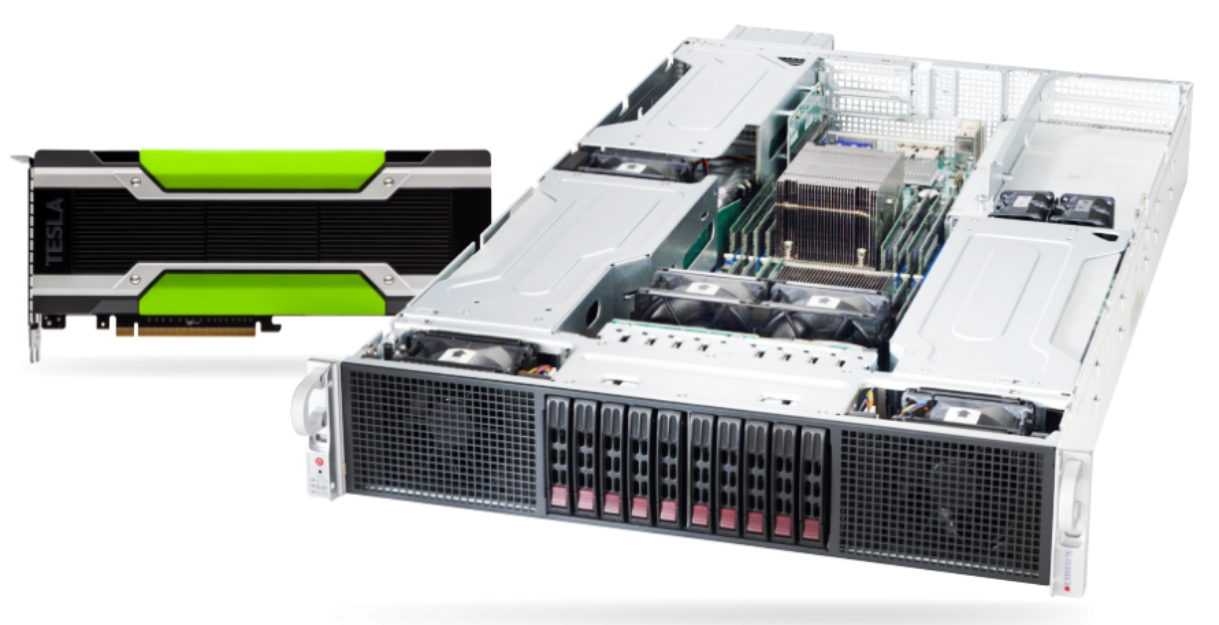
\includegraphics[width=\textwidth]{images/gpx.png}
\end{figure}

\end{frame}

\begin{frame}[fragile]{Bibliography}

\begin{alertblock}{Bibliography}
[1] M. Vinkler and V. Havran, “Register efficient dynamic memory allocator for GPUs” , Computer Graphics Forum, vol. 34, no. 8, pp. 143–154, 2015. [Online]. Available: \url{https://onlinelibrary.wiley.com/doi/abs/10.1111/cgf.12666}

[2] A. Adinetz, “Halloc: A High-Throughput Dynamic Memory Allocator for GPGPU Architectures,” 2014 [Online]. Available:
\url{http://on-demand.gputechconf.com/gtc/2014/presentations/S4271-halloc-high-throughput-dynamic-memory-allocator.pdf. [Accessed: 07-Jan-2019]}
\end{alertblock}

\end{frame}

\end{document}
